\documentclass[10.5pt]{article}
\usepackage[letterpaper, margin=0.6in, top=0.5in, bottom=0.5in]{geometry}
\usepackage{amsmath,amssymb,amsthm}
\usepackage{fancyhdr}
\usepackage{xcolor}
\usepackage{tikz}
\usepackage{enumitem}
\usepackage{tcolorbox}
\usepackage{hyperref}

% Define colors matching instructor board annotations
\definecolor{chalkblue}{RGB}{0, 105, 185}
\definecolor{chalkred}{RGB}{205, 35, 35}
\definecolor{chalkpink}{RGB}{230, 90, 120}
\definecolor{chalkcyan}{RGB}{15, 160, 190}
\definecolor{chalkgreen}{RGB}{20, 130, 50}
\definecolor{boxbg}{RGB}{252, 252, 254}
\definecolor{boxframe}{RGB}{150, 160, 180}

\pagestyle{fancy}
\fancyhf{}
\renewcommand{\headrulewidth}{0pt}
\renewcommand{\footrulewidth}{0pt}

\setlength{\parindent}{0pt}
\setlength{\parskip}{2.5pt}

\begin{document}

% ==============================================================================
% PAGE 1
% ==============================================================================
\noindent \textbf{\large Math 105L} \hfill \textbf{\large Lecture 3-2}\\[1pt]
{\textbf{\Large Intro to Mathematical Modeling: Shapes of Graphs \& Variables}}\\[-5pt]
\rule{\textwidth}{1.2pt}

\vspace{0.03in}

\textbf{\large 1. Thinking About Shapes of Graphs: Partnership Life Proportion}

\begin{tcolorbox}[colback=boxbg, colframe=boxframe, boxrule=0.8pt, arc=3pt, left=8pt, right=8pt, top=4pt, bottom=4pt]
\textbf{Problem Statement:} Suppose that a person meets their future partner at age $18$, that the partner dies when the person is $70$, and that the person then goes on to live to age $100$. If $x$ represents the person's age, draw the graph showing the proportion $P(x)$ of their life that they have been with their partner. Then write down a formula for $P(x)$, showing all your work.
\end{tcolorbox}

\vspace{0.04in}

\textbf{Mathematical Formulation \& Formula Derivation:}
\begin{itemize}[leftmargin=1.2em, topsep=1pt, itemsep=2pt]
  \item \textbf{Phase 1 ($x < 18$):} The person has not yet met their partner. The time spent together is $0$.
  \[
  P(x) = 0
  \]
  \item \textbf{Phase 2 ($18 \le x \le 70$):} The person met their partner at age $18$. At age $x$, the total number of years spent together is $x - 18$. The person's total lifetime lived to date is $x$. Therefore, the proportion is:
  \[
  P(x) = \frac{x - 18}{x} = 1 - \frac{18}{x}
  \]
  \item \textbf{Phase 3 ($70 < x \le 100$):} The partner died at age $70$. The total time spent together is frozen at $70 - 18 = 52$ years. The person continues to age to $x$. Therefore, the proportion of their life spent together is:
  \[
  P(x) = \frac{52}{x}
  \]
\end{itemize}

\begin{tcolorbox}[colback=white, colframe=chalkblue, boxrule=1pt, arc=3pt, left=10pt, right=10pt, top=4pt, bottom=4pt]
\[
P(x) = \begin{cases}
0 & \text{if } x < 18 \\[4pt]
\dfrac{x - 18}{x} = 1 - \dfrac{18}{x} & \text{if } 18 \le x \le 70 \\[6pt]
\dfrac{52}{x} & \text{if } 70 < x \le 100
\end{cases}
\]
\end{tcolorbox}

\vspace{0.03in}
\textbf{Graph Analysis \& Justification of Concavity:}
\begin{center}
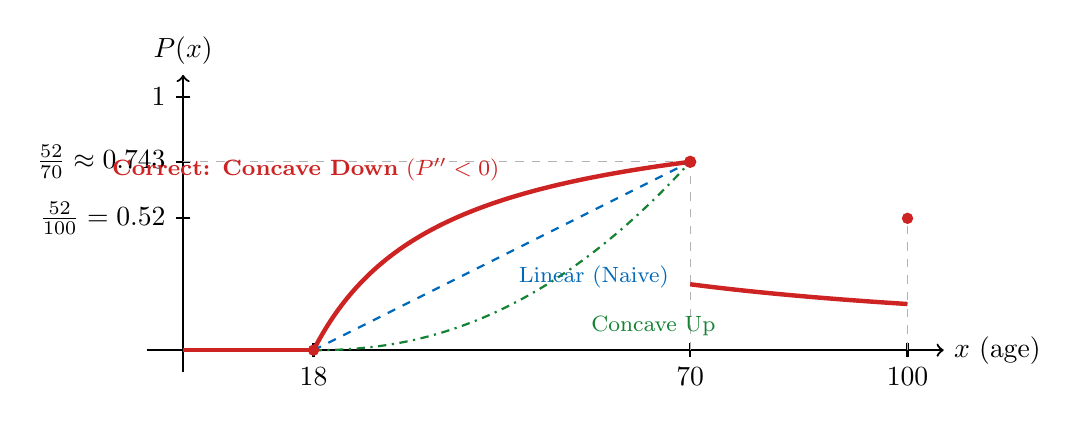
\begin{tikzpicture}[scale=0.92]
  % Axes
  \draw[->, thick] (-0.5, 0) -- (10.5, 0) node[right] {$x$ (age)};
  \draw[->, thick] (0, -0.3) -- (0, 3.8) node[above] {$P(x)$};

  % Ticks on x-axis
  \draw[thick] (1.8, 0.1) -- (1.8, -0.1) node[below] {$18$};
  \draw[thick] (7.0, 0.1) -- (7.0, -0.1) node[below] {$70$};
  \draw[thick] (10.0, 0.1) -- (10.0, -0.1) node[below] {$100$};

  % Ticks on P-axis
  \draw[thick] (0.1, 3.5) -- (-0.1, 3.5) node[left] {$1$};
  \draw[thick] (0.1, 2.6) -- (-0.1, 2.6) node[left] {$\frac{52}{70} \approx 0.743$};
  \draw[dashed, gray!60] (0, 2.6) -- (7.0, 2.6);
  \draw[dashed, gray!60] (7.0, 0) -- (7.0, 2.6);

  % Flat before 18
  \draw[ultra thick, chalkred] (0, 0) -- (1.8, 0);

  % Three candidate curves discussed on blackboard between 18 and 70:
  % Red: Concave Down (Correct)
  \draw[ultra thick, chalkred, domain=1.8:7.0, samples=80] plot (\x, {3.5 * (1 - 1.8/\x)});
  % Blue: Linear (Incorrect naive guess)
  \draw[thick, chalkblue, dashed] (1.8, 0) -- (7.0, 2.6);
  % Green: Concave Up (Incorrect)
  \draw[thick, chalkgreen, dashdotted, domain=1.8:7.0, samples=80] plot (\x, {2.6 * ((\x - 1.8)/5.2)^2.2});

  % After 70: 52/x
  \draw[ultra thick, chalkred, domain=7.0:10.0, samples=60] plot (\x, {3.5 * (1.82 / \x)});
  \draw[dashed, gray!60] (10.0, 0) -- (10.0, 1.82);
  \draw[thick] (0.1, 1.82) -- (-0.1, 1.82) node[left] {$\frac{52}{100} = 0.52$};

  % Points
  \filldraw[chalkred] (1.8, 0) circle (2pt);
  \filldraw[chalkred] (7.0, 2.6) circle (2.2pt);
  \filldraw[chalkred] (10.0, 1.82) circle (2pt);

  % Labels
  \node[chalkred, font=\footnotesize, above left] at (4.5, 2.2) {\textbf{Correct: Concave Down} ($P'' < 0$)};
  \node[chalkblue, font=\footnotesize, below right] at (4.5, 1.3) {Linear (Naive)};
  \node[chalkgreen, font=\footnotesize, below right] at (5.5, 0.6) {Concave Up};
\end{tikzpicture}
\end{center}

\vspace{-0.05in}
\begin{itemize}[leftmargin=1.2em, topsep=1pt, itemsep=2pt]
  \item \textbf{Why is $P(x)$ concave down on $[18, 70]$?}
  Taking derivatives of $P(x) = 1 - 18 x^{-1}$:
  \[
  P'(x) = \frac{18}{x^2} > 0 \quad (\text{strictly increasing}), \qquad P''(x) = -\frac{36}{x^3} < 0 \quad (\text{strictly concave down}).
  \]
  \textit{Intuitive Reasoning:} Immediately after meeting at age $18$, each additional year lived adds a massive fraction to the proportion. By age $36$ (just $18$ years later), the person has spent $18/36 = 50\%$ of their life with their partner. But in later years, adding one year increases the fraction only marginally (at age $69 \to 70$, the change is under $0.4\%$). Thus, the rate of increase slows down, producing a concave down curve.
  \item \textbf{Why does $P(x)$ decrease and curve concave up on $(70, 100]$?}
  $P'(x) = -52 x^{-2} < 0$ and $P''(x) = 104 x^{-3} > 0$. The proportion dilutes toward zero as the total lifespan $x$ grows while the shared years remain fixed at $52$.
\end{itemize}

\newpage

% ==============================================================================
% PAGE 2
% ==============================================================================
\noindent \textbf{\large Math 105L \hfill Lecture 3-2 (Continued)}\\[-5pt]
\rule{\textwidth}{1.2pt}

\vspace{0.04in}

\textbf{\large 2. Qualitative Modeling: Contagious Disease Epidemic}

\begin{tcolorbox}[colback=boxbg, colframe=boxframe, boxrule=0.8pt, arc=3pt, left=8pt, right=8pt, top=4pt, bottom=4pt]
\textbf{Problem 1:} Consider a situation in which a contagious disease is spreading through a city of $1,000,000$ people. Assume also that:
\begin{enumerate}[label=(\alph*), topsep=1pt, itemsep=1pt]
  \item no one (or almost no one) dies from the disease,
  \item once one recovers from it, one doesn't get the disease again (permanent immunity),
  \item the epidemic runs its course in a one month ($30$ day) period,
  \item $20\%$ of the population never gets the disease, and
  \item the epidemic begins with one person ($N(0) = 1$).
\end{enumerate}
Draw a possible graph that gives the number of people who have \emph{contracted} the disease during the epidemic as a function of time. Label axes carefully (including scales) and justify the shape of the graph.
\end{tcolorbox}

\vspace{0.04in}
\begin{center}
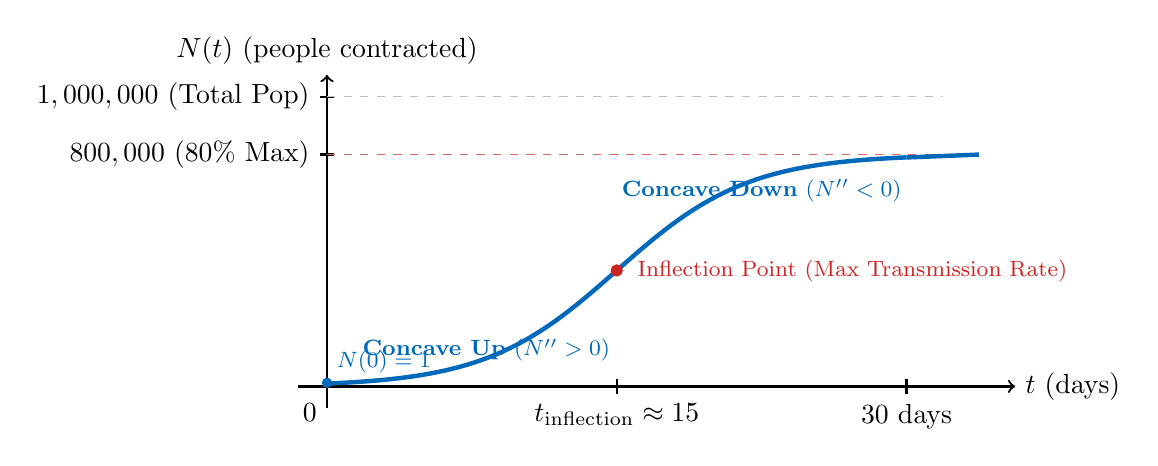
\begin{tikzpicture}[scale=0.92]
  % Axes
  \draw[->, thick] (-0.4, 0) -- (9.5, 0) node[right] {$t$ (days)};
  \draw[->, thick] (0, -0.3) -- (0, 4.3) node[above] {$N(t)$ (people contracted)};

  % Ticks on t-axis
  \draw[thick] (0, 0.1) -- (0, -0.1) node[below left] {$0$};
  \draw[thick] (4.0, 0.1) -- (4.0, -0.1) node[below] {$t_{\text{inflection}} \approx 15$};
  \draw[thick] (8.0, 0.1) -- (8.0, -0.1) node[below] {$30$ days};

  % Ticks on N-axis
  \draw[thick] (0.1, 4.0) -- (-0.1, 4.0) node[left] {$1,000,000$ (Total Pop)};
  \draw[dashed, gray!50] (0, 4.0) -- (8.5, 4.0);

  \draw[thick] (0.1, 3.2) -- (-0.1, 3.2) node[left] {$800,000$ ($80\%$ Max)};
  \draw[dashed, chalkred!70] (0, 3.2) -- (8.5, 3.2);

  % Logistic S-curve
  \draw[ultra thick, chalkblue, domain=0:8.0, samples=80] plot (\x, {3.2 / (1 + exp(-1.1 * (\x - 4.0)))});
  \draw[ultra thick, chalkblue] (8.0, 3.16) -- (9.0, 3.2);

  % Inflection point
  \filldraw[chalkred] (4.0, 1.6) circle (2.2pt) node[right=4pt, chalkred, font=\footnotesize] {Inflection Point (Max Transmission Rate)};
  \filldraw[chalkblue] (0, 0.05) circle (1.8pt) node[above right, font=\footnotesize] {$N(0) = 1$};

  % Region labels
  \node[font=\footnotesize, chalkblue] at (2.2, 0.5) {\textbf{Concave Up} ($N'' > 0$)};
  \node[font=\footnotesize, chalkblue] at (6.0, 2.7) {\textbf{Concave Down} ($N'' < 0$)};
\end{tikzpicture}
\end{center}

\vspace{-0.05in}
\textbf{Detailed Justification of the $S$-Shape (Logistic Growth):}
\begin{itemize}[leftmargin=1.2em, topsep=1pt, itemsep=2pt]
  \item \textbf{Initial Condition \& Cumulative Measure:} $N(t)$ measures total people who have \emph{contracted} the disease. Since no one loses contracted status (immunity means they don't get it again, and no one dies), $N(t)$ is strictly non-decreasing ($N'(t) \ge 0$). At $t = 0$, $N(0) = 1 \approx 0$.
  \item \textbf{Early Exponential Phase (Concave Up, $N'' > 0$):} Initially, almost the entire city is susceptible ($999,999$ people). As the number of infected individuals grows, there are more transmitters interacting with a virtually unlimited pool of susceptible hosts. The number of new daily infections accelerates, so the slope steepens ($N'' > 0$).
  \item \textbf{Inflection Point (Peak Spread Rate):} Around the middle of the month (approximately day $15$), the spread rate $dN/dt$ reaches its maximum.
  \item \textbf{Late Saturation Phase (Concave Down, $N'' < 0$):} As the number of contracted individuals approaches the threshold of $800,000$ ($80\%$ of $1,000,000$), infected people encounter fewer and fewer susceptible people. The spread decelerates, causing the curve to become concave down ($N'' < 0$) and level off asymptotically toward $800,000$.
  \item \textbf{Endpoint ($t = 30$):} At $t = 30$ days, the epidemic has run its course, meaning new infections drop to $0$ and the graph flattens horizontally at exactly $N = 800,000$.
\end{itemize}

\vspace{0.08in}

\textbf{\large 3. Playing with Variables: Gas Mileage \& Travel Optimization}

\begin{tcolorbox}[colback=boxbg, colframe=boxframe, boxrule=0.8pt, arc=3pt, left=8pt, right=8pt, top=4pt, bottom=4pt]
\textbf{Problem 2:} Suppose you have a car that gets $24$ miles per gallon and you are going to buy $10$ gallons of gas. A gas station near you sells gas for $\$2.499/\text{gal}$, but one $4$ miles down the road sells gas for $\$2.459/\text{gal}$. Assuming gas is the only cost:
\begin{enumerate}[label=(\alph*), topsep=1pt, itemsep=1pt]
  \item Would you save money by driving the extra $4$ miles?
  \item What if the gas station were only $1$ mile away?
  \item What is the least distance at which you would \emph{not} save any money?
\end{enumerate}
\end{tcolorbox}

\vspace{0.03in}
\textbf{General Algebraic Cost Model:}
Let $D$ be the one-way distance to the further gas station (miles).
\begin{itemize}[leftmargin=1.2em, topsep=1pt, itemsep=2pt]
  \item Near station cost: $C_{\text{near}} = 10 \text{ gal} \times \$2.499/\text{gal} = \mathbf{\$24.99}$.
  \item Round-trip distance to further station: $2D$ miles.
  \item Gas consumed on round-trip: $\dfrac{2D \text{ miles}}{24 \text{ mpg}} = \dfrac{D}{12} \text{ gallons}$.
  \item Total gas purchased: To end up with $10$ net gallons in the tank, you must purchase $10 + \dfrac{D}{12}$ gallons at $\$2.459/\text{gal}$:
  \[
  C_{\text{far}}(D) = \left(10 + \frac{D}{12}\right) \times 2.459 = 24.59 + \left(\frac{2.459}{12}\right) D \approx 24.59 + 0.204917 D
  \]
\end{itemize}

\textbf{Solutions to Subquestions:}
\begin{enumerate}[label=(\alph*), leftmargin=1.2em, topsep=1pt, itemsep=3pt]
  \item \textbf{Distance $D = 4$ miles:}
  \[
  C_{\text{far}}(4) = 24.59 + \frac{4}{12} \times 2.459 = 24.59 + \frac{2.459}{3} \approx 24.59 + 0.82 = \mathbf{\$25.41}
  \]
  Since $\$25.41 > \$24.99$, you would \textbf{lose} $\$0.42$. \textbf{No, you do not save money.}
  \item \textbf{Distance $D = 1$ mile:}
  \[
  C_{\text{far}}(1) = 24.59 + \frac{1}{12} \times 2.459 \approx 24.59 + 0.205 = \mathbf{\$24.795} \approx \mathbf{\$24.80}
  \]
  Since $\$24.80 < \$24.99$, you \textbf{save} approximately $\$24.99 - \$24.795 = \mathbf{\$0.195}$ ($\approx 20\text{ cents}$). \textbf{Yes, you save money.}
  \item \textbf{Break-Even Distance $D^*$:}
  Set $C_{\text{far}}(D^*) = C_{\text{near}}$:
  \[
  24.59 + 0.204917 D^* = 24.99 \implies 0.204917 D^* = 0.40 \implies D^* = \frac{0.40}{0.204917} = \frac{0.40 \times 12}{2.459} \approx \mathbf{1.952 \text{ miles}}
  \]
  \textbf{Conclusion:} At any distance $D \ge \mathbf{1.95 \text{ miles}}$, you will \textbf{not} save any money.
\end{enumerate}

\end{document}
